%\casesection{Flow over a thin wall\label{case:wallflow}}
\section{Flow over a thin wall}


\paragraph*{Purpose}
The purpose of this validation study is to investigate the performance of D-Flow FM for flow over a wall. In the current case, two-dimensional flow with a physically present wall is considered; 'physically' in the sense that the wall is represented within the bathymetry. The case described below is a variant to the Delft3D testcase 3.1.7 from the Delft3D validation document.



\paragraph*{Linked claims}
Claims that are related to the current test case are:
\begin{itemize}
\item claim [empty]: yet to be filled.
\end{itemize}




\paragraph*{Approach}
The flow condition over a wall may be sub- or supercritical. For supercritical flow, the discharge at the wall is completely determined by the energy head upstream. In such a case, the discharge is limited by:
\begin{equation}
Q_{critical} = B\frac{2}{3}E_{up}\sqrt{\frac{2}{3}gE_{up}}.
\end{equation}
The purpose of this validation study is to verify whether D-Flow FM is able to accurately compute this theoretical maximum. For this testcase, the wall is presented within the bathymetry. Both a coarse grid and a finer grid are considered.

%In D-Flow FM multiple advection schemes have been implemented. By means of mutual comparison of the several advection schemes, it is examined to what extent D-Flow FM is able to simulate flow over a wall.





\paragraph*{Model description}
The upstream water level boundary is 2.0 m and the downstream boundary equals 1.7 m. The wall height is 1.0 m above the bottom of the channel. The discharge is critical over the top of the wall. The energy height upstream $E_{up}$ is about 1.0 m. The width $B$ of the channel is 90 m. The Ch\'ezy coefficient is 100 m$^{1/2}$/s. The channel is simulated on a grid with cell sizes equal to 10 m $\times$ 10 m and 30 m $\times$ 30 m, respectively. 

\begin{figure}[h!]
\begin{center}
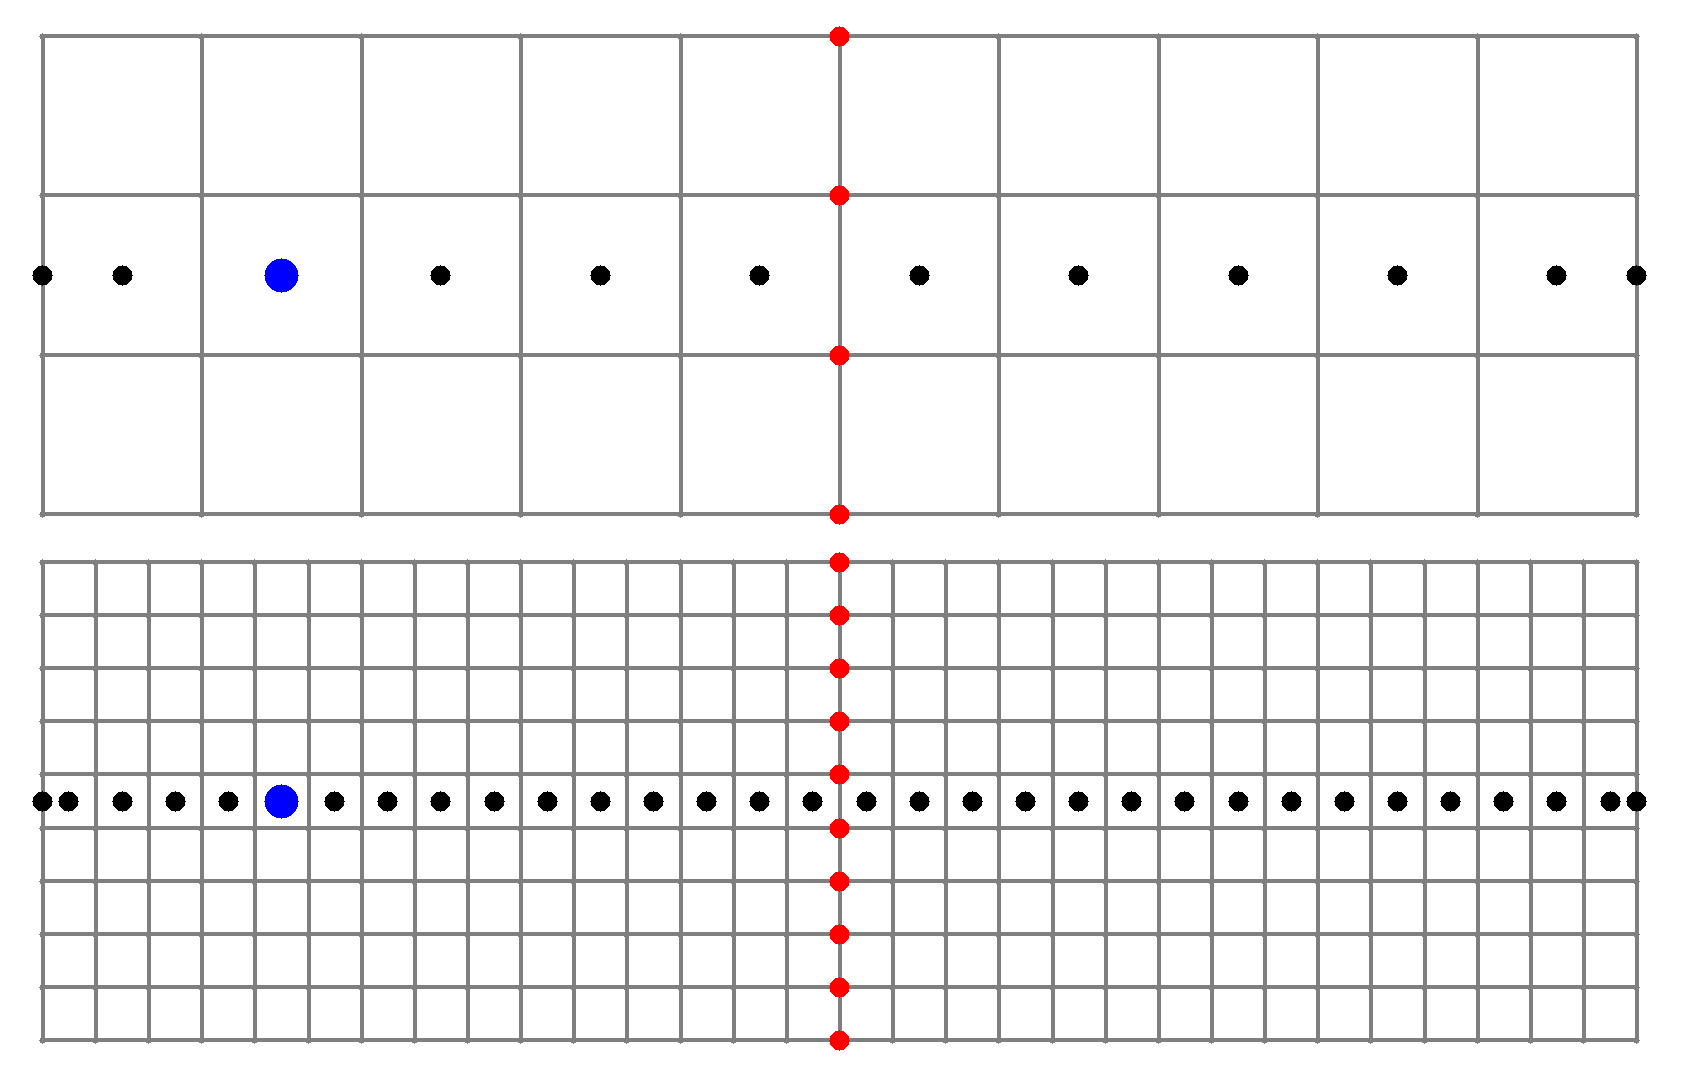
\includegraphics[width=0.74\columnwidth]{figures/gridswithweirandobs.png}
\end{center}\caption{Computational grids for the flow over a wall. The bed level is 0.0 m (w.r.t. reference), except the locations marked by red dot, at which the bed level is 1.0 m (w.r.t. reference). The flow is from left to right. The thick blue dot marks the observation point used to study the output timeseries for. \label{fig:gridswithwallandobs}}
\end{figure}

On the coarse grid the wall is represented by one grid cell and on the fine grid by three grid cells (as illustrated in \Fref{fig:gridswithwallandobs}). For this test case $Q_{critical}$ yields a maximum discharge of 153 m$^3$/s. The location of the outflow water levels is set on the exact, actual boundary of the grid, which prevents the necessity to adapt the value of the outflow water level for the grid staggering.





\paragraph*{Results}
\Fref{fig:wallresult} shows the spatial development of the water levels in longitudinal direction. Considerable differences can be observed between the results on the coarse grid on the one hand and on the fine grid on the other hand. For this picture, advection scheme number 3 (assigned as \texttt{Perot q(uio-u)}) is used.

\begin{figure}[h!]
\begin{center}
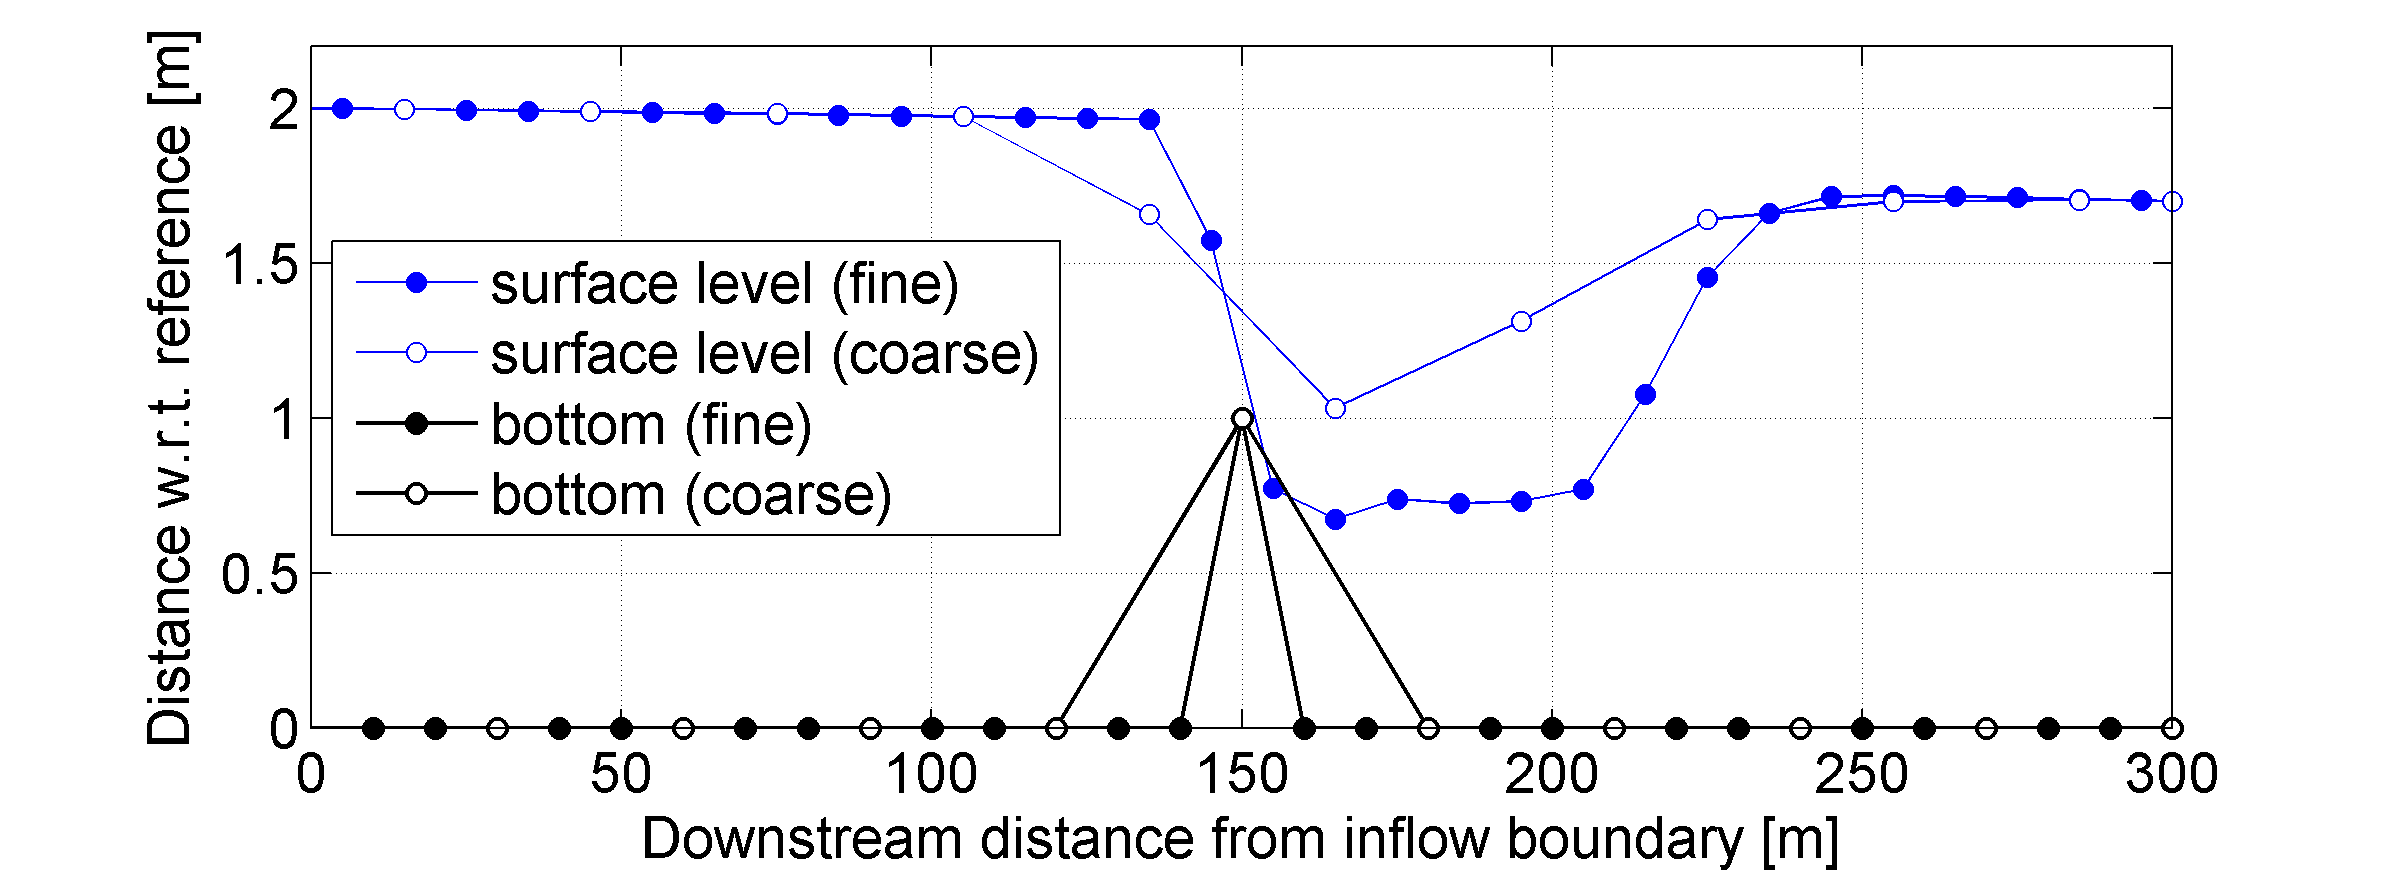
\includegraphics[width=0.9\columnwidth]{figures/weirresult.png}
\end{center}\caption{Computed water levels for flow over a wall, both on a coarse grid (with grid sizes of 30 m) and a fine grid (with grid sizes of 10 m). \label{fig:wallresult}}
\end{figure}

For some advection schemes, discharges $Q$ have been computed. The computed values of $Q$ are given in \Tref{tab:advecdischarges}. The computed values show significant differences, both mutually between the grids and mutually between the advection schemes. Furthermore, the coarse grid cases overpredict the discharge by a factor of 2 (roughly), whereas the fine grid cases overpredict the discharge by a about 40\%.

\begin{table}[h!]
\centering
\caption{Computed discharge $Q$ for several advection schemes, both for the coarse grid and the fine grid. The name of the advection scheme is taken from the \texttt{mdu}-file.}
\label{tab:advecdischarges}
\begin{tabular}{r p{6cm} r r} \hline
   & Advection schemes           & $Q$ [m$^3$/s] (coarse)  &  $Q$ [m$^3$/s] (fine) \\ \hline \hline
1 & \texttt{Wenneker, qu-udzt}                   & 396  &  208   \\
2 & \texttt{1, q(uio-u)}                         & 362  &  194   \\
3 & \texttt{Perot q(uio-u)}                      & 364  &  361   \\
4 & \texttt{Perot q(ui-u)}                       & 440  &  251   \\ 
5 & \texttt{Perot q(ui-u) without itself}        & 362  &  194   \\ \hline
\end{tabular}
\end{table}

For advection scheme number 3, some timeseries are considered in more detail. The location of this further analysis is chosen downstream of the wall (marked by the blue dot in \Fref{fig:gridswithwallandobs}). The computed timeseries for the water levels and streamwise velocities are shown in \Fref{fig:wallseries}.

The left panel of \Fref{fig:wallseries} shows that the water levels computed on both the grids more or less coincide. However, for the fine grid, small wiggles are observed for the water level. The right panel of \Fref{fig:wallseries} shows that for the coarse grids the velocities are almost twice as high as for the fine grids. On the other hand, for the fine grid, considerable wiggles are observed for the streamwise velocities

\begin{figure}[h!]
\begin{center}
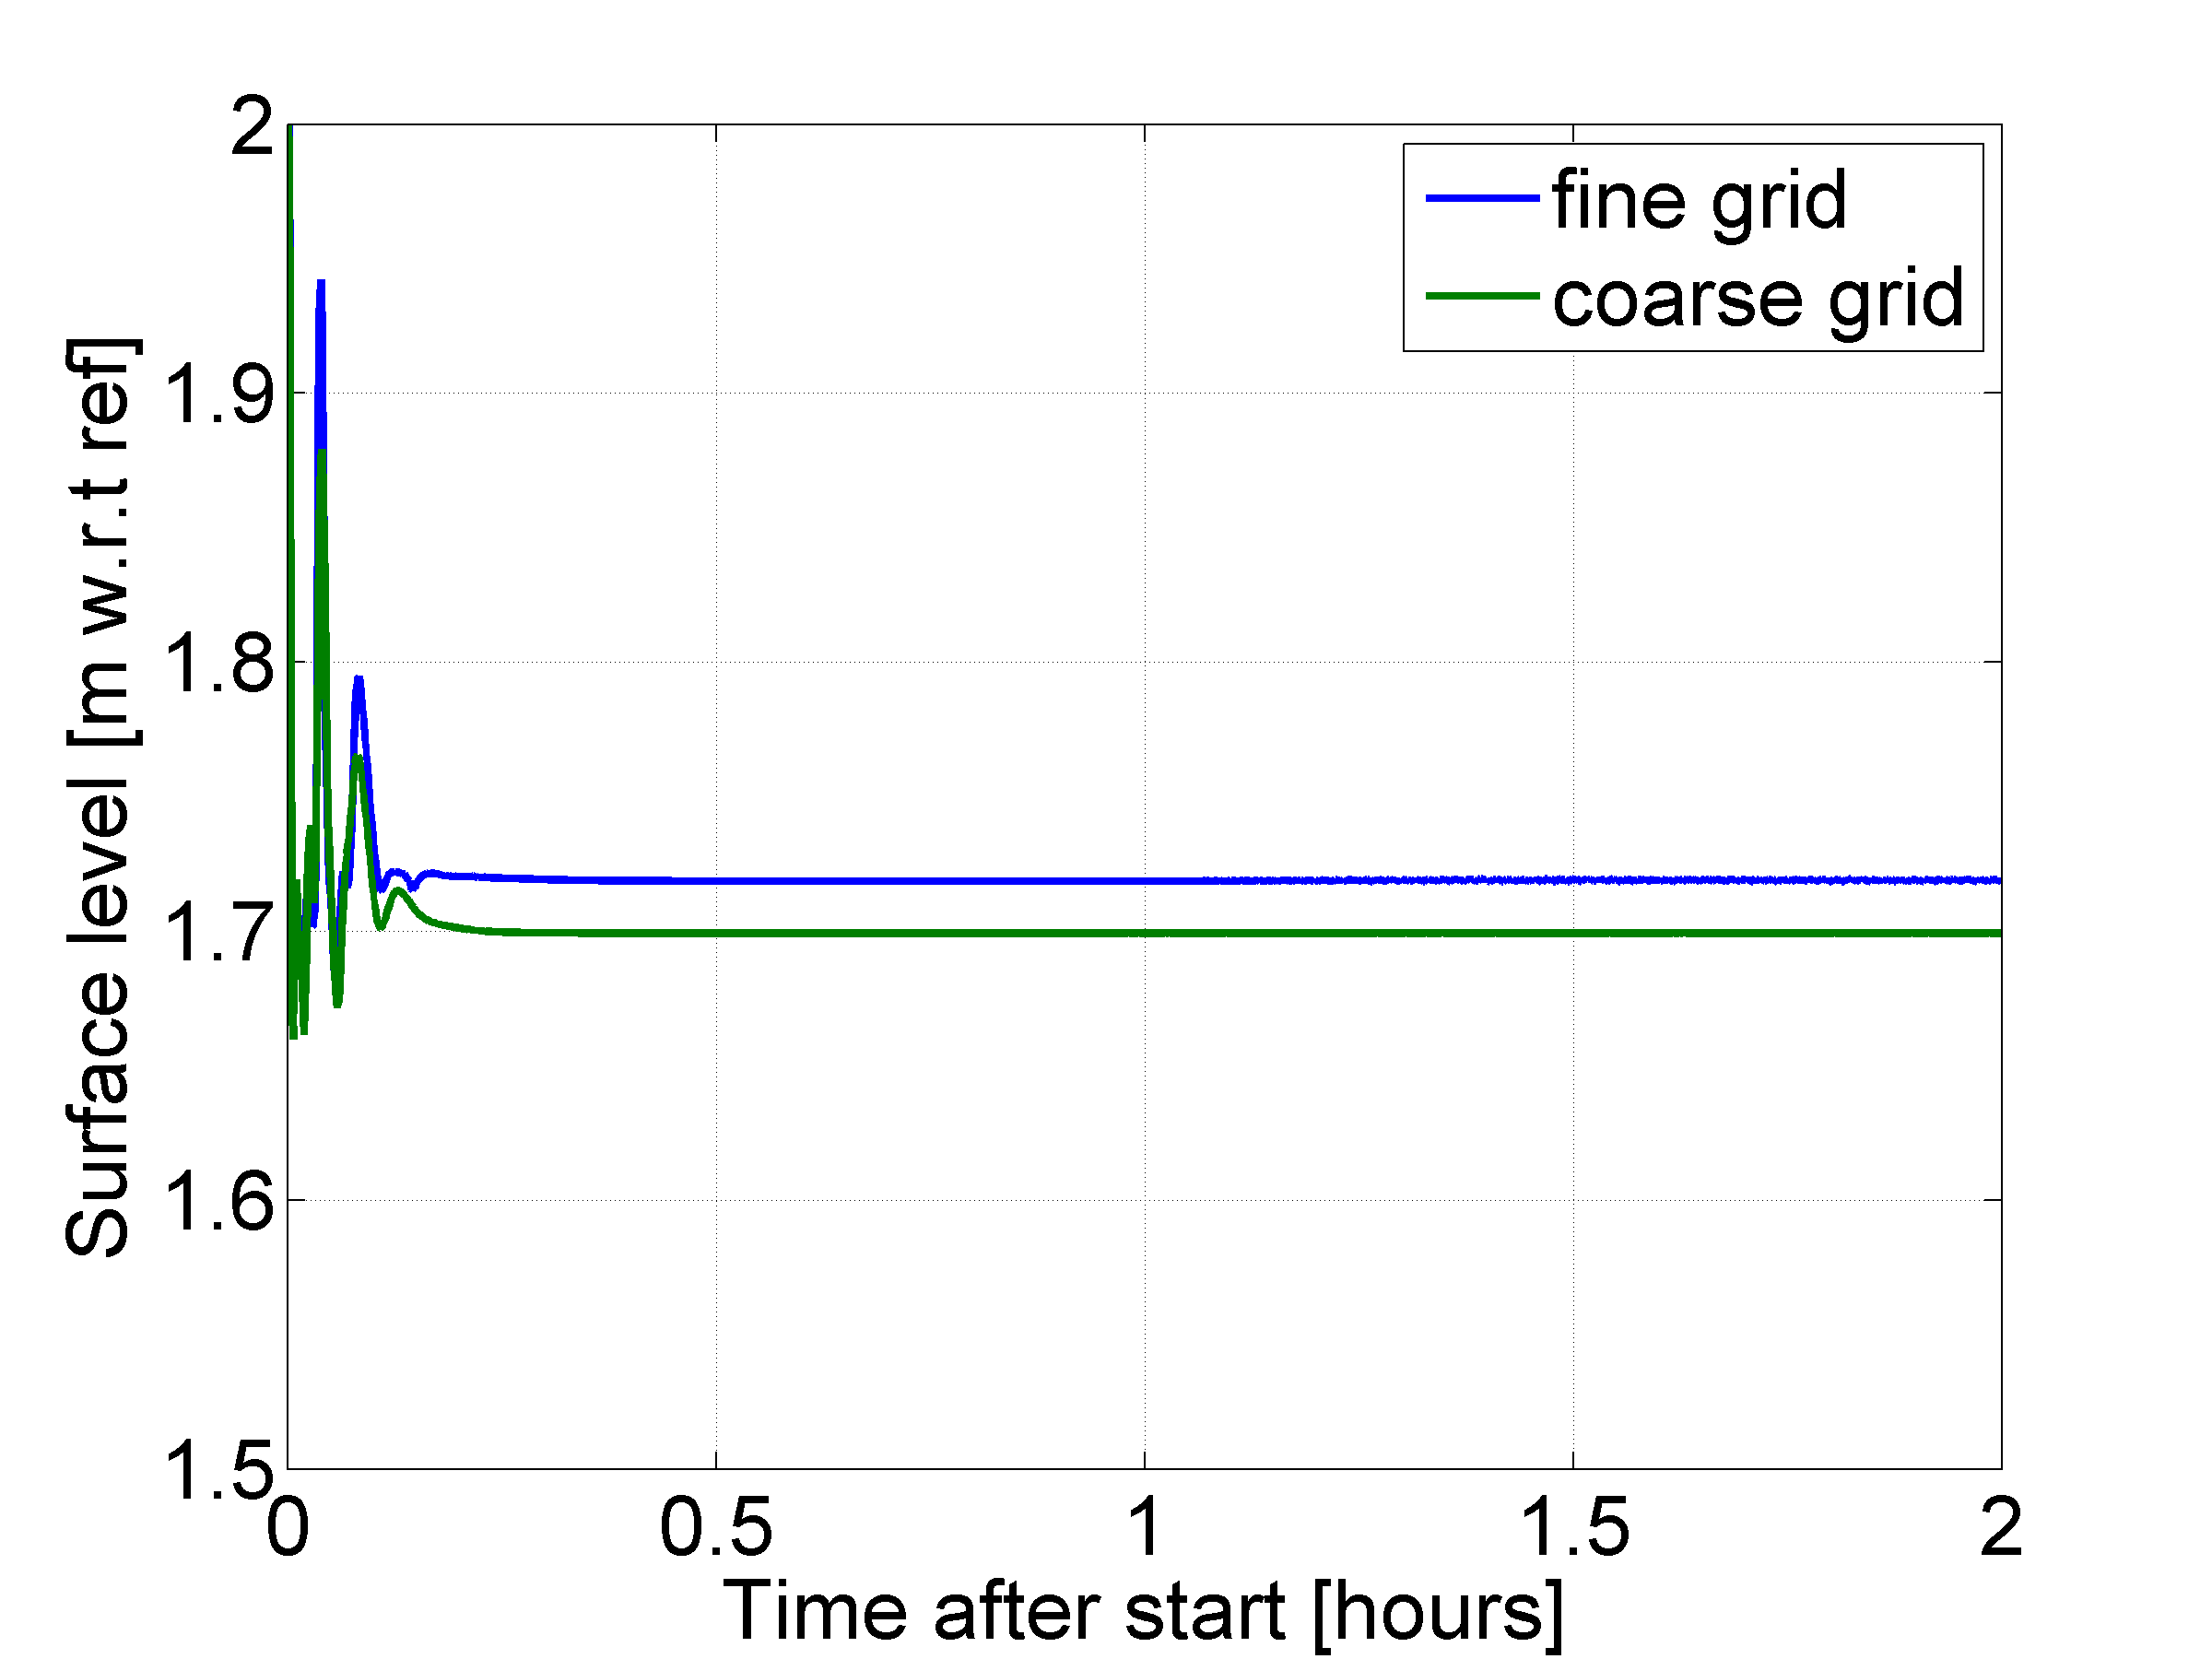
\includegraphics[width=0.49\columnwidth]{figures/waterlevels.png}
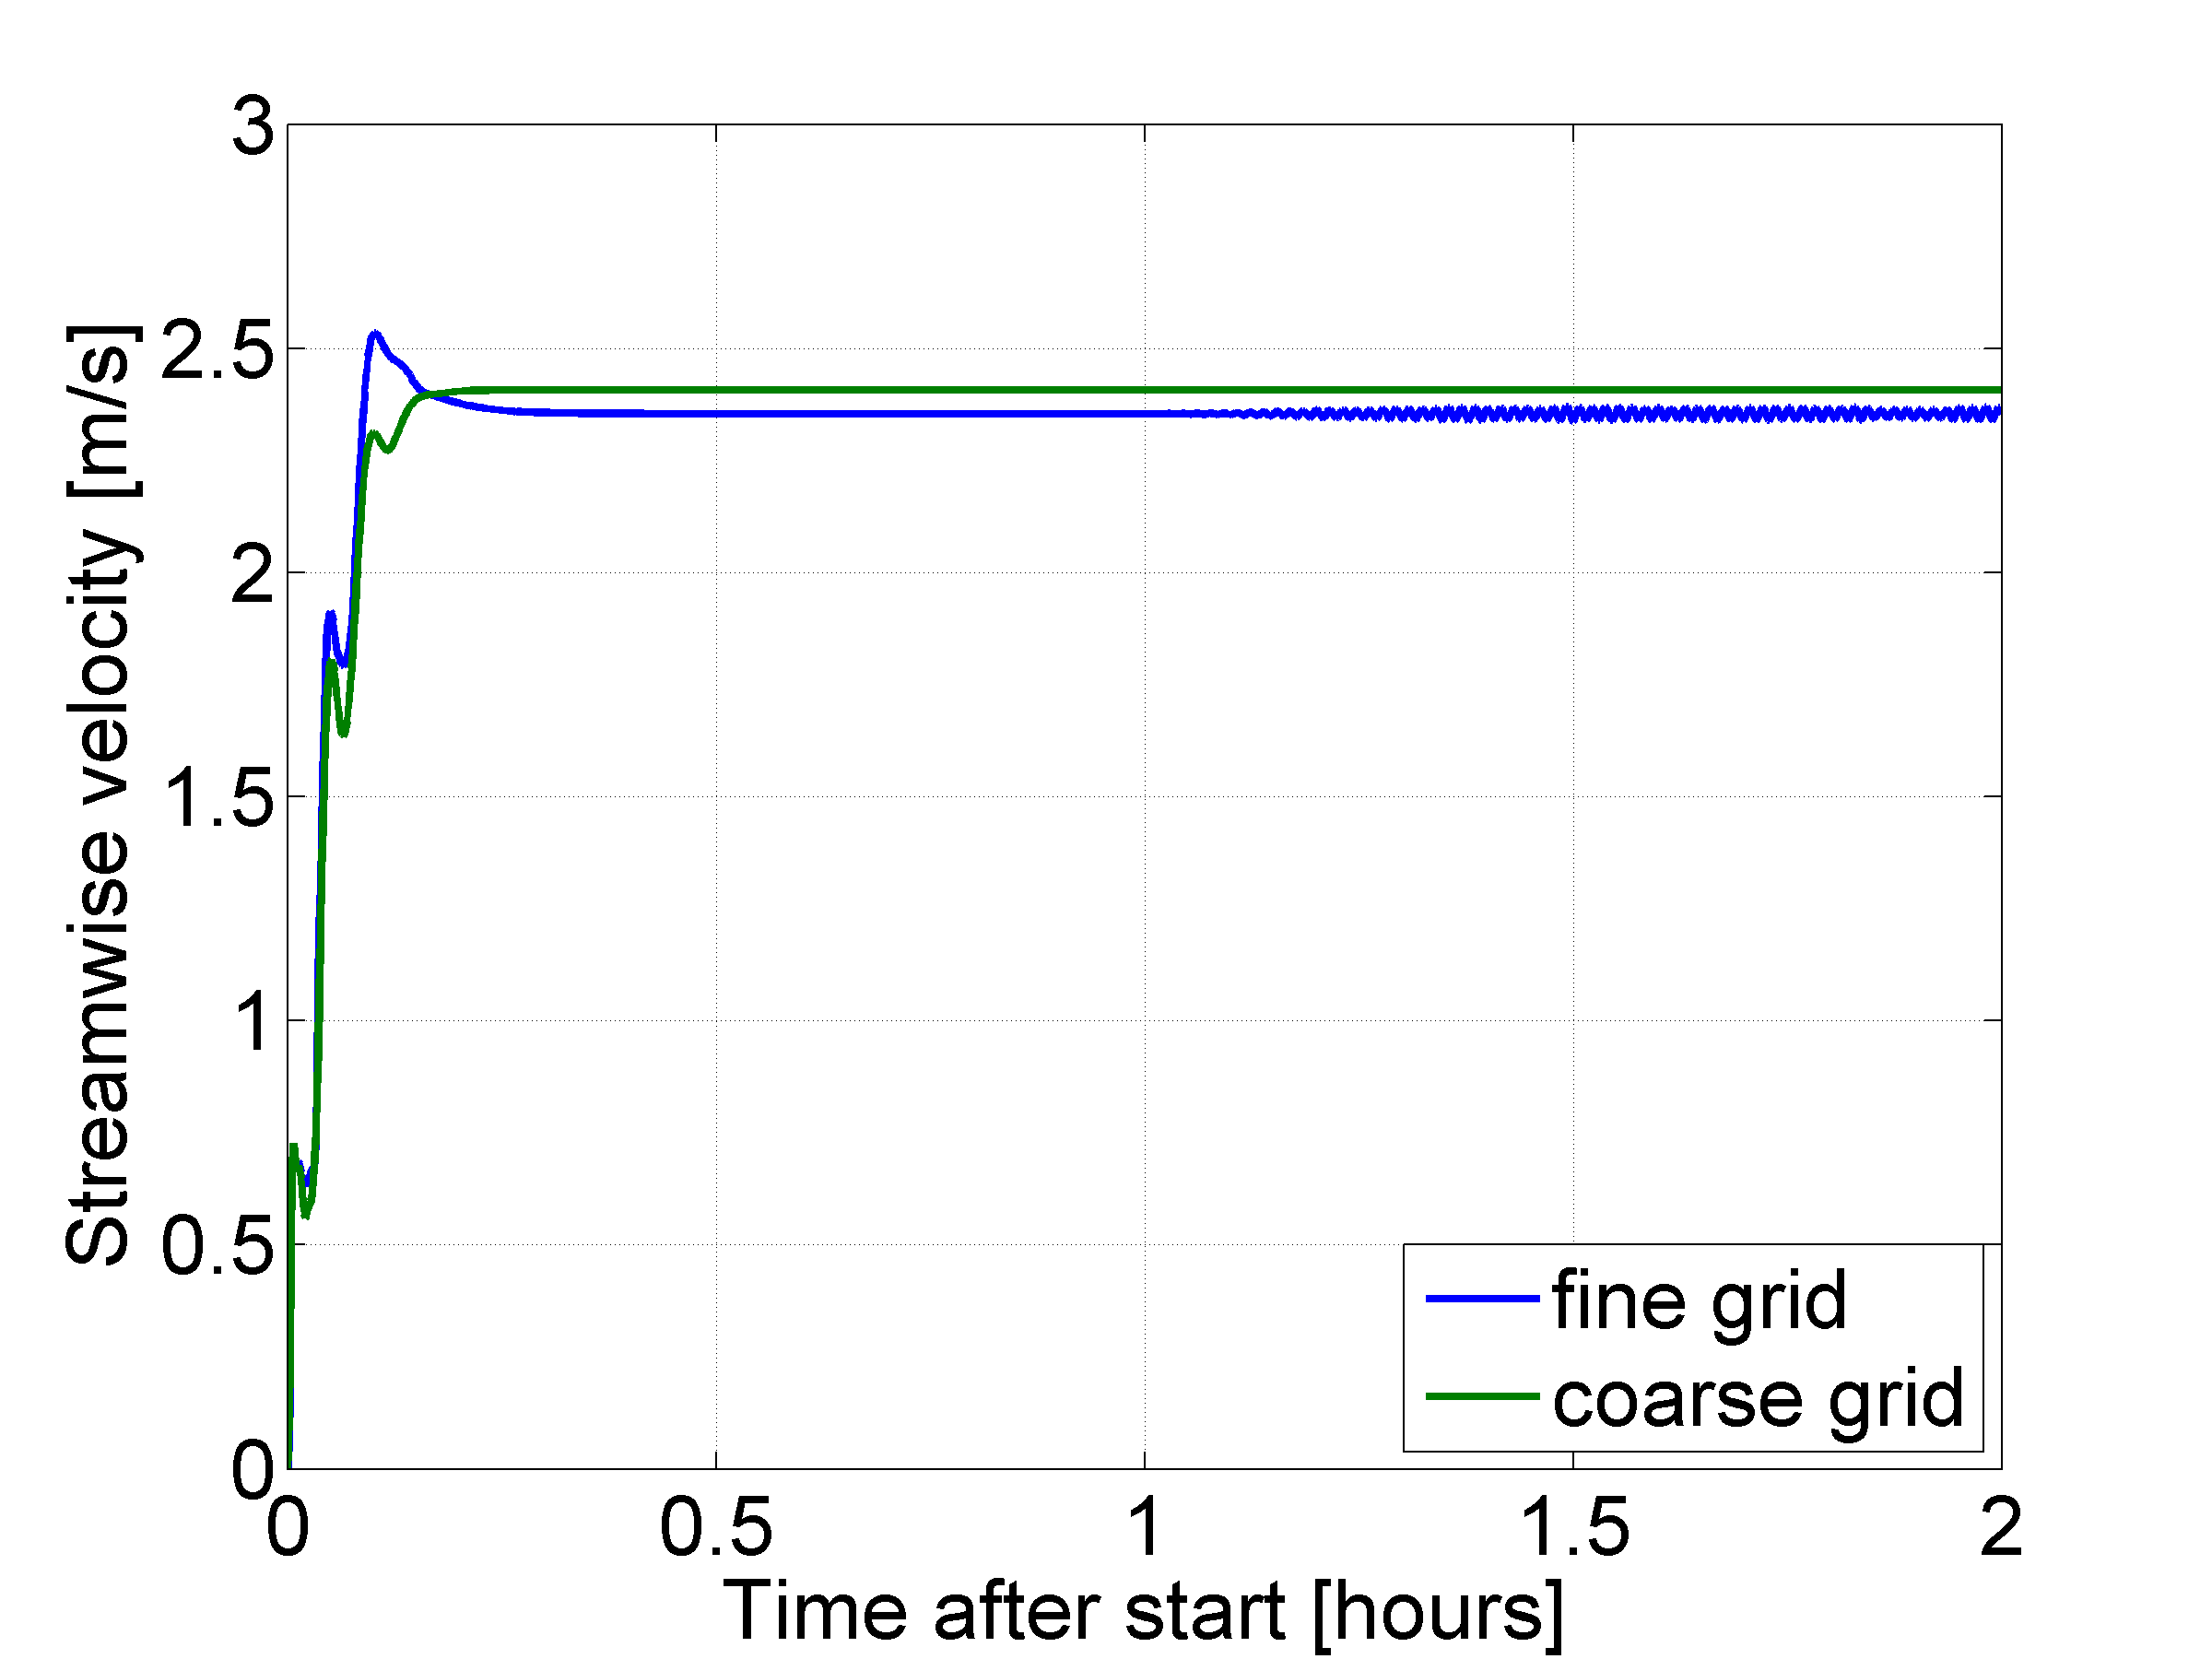
\includegraphics[width=0.49\columnwidth]{figures/velocities.png}
\end{center}\caption{Left panel: computed water levels for the coarse grid and the fine grid, downstream of the wall. Right panel: computed streamwise velocities for the coarse grid and the fine grid, downstream of the wall). \label{fig:wallseries}}
\end{figure}






\paragraph*{Conclusions}
Considerable differences are observed in the results for flow over a wall, when considering two grades of the grid resolution and five types of advection schemes. Both the coarse grid and the fine grid significantly deviate from the analytical outcome. Moreover, spurious velocity oscillations are found for the fine grid, downstream of the wall. 


\paragraph*{Version}
This test has been carried out with version dflow-fm-x64-1.1.90.31666.